% !TEX root = main.tex


\secmoveup
\section{Experiments}
This section describes settings for neural network learning, baselines and
evaluation metrics, followed by a discussion of key results.


\secmoveup
\subsection{Training Details}
\label{ssec:training_details}

% \verify{MOST OF THIS IS ABOUT THE COPYING MECHANISM REMOVE? To
% 	train the full model, we first freeze all the encoder weights
% 	and remove the copying mechanism. We then train the decoder by minimising the
% 	negative log likelihood of the correct token at each time step. Once the model
% 	has converged, we freeze the newly trained weights, add the
% 	copying mechanism, and minimize the loss of copying the proper nouns. The loss
% 	for copying proper nouns is the sum of the binary cross-entropy loss for $p(c)$ and
% 	the categorical cross-entropy of the attention weights $\lambda_i$ on the
% 	proper nouns in the article text. This is fully supervised as we label all the
% 	proper nouns in the articles and training caption using the NLP package
% 	SpaCy~\cite{spacy2}.}

% Note that given kernel size $K$, we can attend to the current time step and
% the last $K-1$ steps. Thus the final block output will have collected
% information from the last 51 tokens.

Following Wu \etal~\cite{Wu2018PayLA}, we set the hidden size $D^E$ to 1024;
the number of heads $H$ to 16; and the number of transformer blocks $L$ to four
with kernel sizes 3, 7, 15, and 31, respectively. For parameter optimization we
use the adaptive gradient algorithm Adam~\cite{Kingma2015Adam} with the
following parameter: $\beta_1 = 0.9, \beta_2 = 0.98, \epsilon = 10^{-6}$. We
warm up the learning rate in the first 5\% of the training steps to $10^{-4}$,
and decay it linearly afterwards. We apply $L_2$ regularization to all network
weights with a weight decay of $10^{-5}$ and using the
fix~\cite{Loshchilov2018DecoupledWD} that decouples the learning rate from the
regularization parameter. We clip the gradient norm at 0.1. We use a maximum
batch size of 16 and training is stopped after the model has seen 6.6 million
examples. This is equivalent to 16 epochs on GoodNews and 9 epochs on
NYTimes800k.



The training pipeline is written in PyTorch~\cite{Paszke2017Automatic} using
the AllenNLP framework~\cite{Gardner2017AllenNLP}. The RoBERTa model and
dynamic convolution code are adapted from fairseq~\cite{Ott2019Fairseq}.
Training is done with mixed precision to reduce the memory footprint and allow
our full model to be trained on a single GPU. The full model takes 5 days to
train on one Titan V GPU and has 200 million trainable parameters---see the
supplementary material for the size of each model variant.

\secmoveup
\subsection{Evaluation Metrics}

We use BLEU-4~\cite{Papineni2002Bleu} and CIDEr~\cite{Vedantam2015CIDEr} scores
as they are standard for evaluating image captions. These are obtained using
the COCO caption evaluation
toolkit\footnote{\href{https://github.com/tylin/coco-caption}
{https://github.com/tylin/coco-caption}}. The supplementary material
additionally reports BLEU-1, BLEU-2, BLEU-3, ROUGE \cite{Lin2004ROUGE}, and
METEOR~\cite{Denkowski2014Meteor}. Note that CIDEr is particularly suited for
evaluating news captioning models as it puts more weight than other metrics on
uncommon words. In addition, we evaluate the precision and recall on named
entities, people's names, and rare proper names. Named entities are identified
in both the ground-truth captions and the generated captions using SpaCy. We
then count exact string matches between the ground truths and generated
entities. For people's names we restrict the set of named entities to those
marked as PERSON by the SpaCy parser. Rare proper nouns are nouns that appear
in a test caption but not in any training caption.


\begin{table}[t]
	\caption {NYTimes800k training, validation, and test splits}
	\label{tab:splits}
	\centering
	\begin{tabularx}{\linewidth}{lXXX}
		\toprule
		  & Training  &   Validation & Test \\
		\midrule
      Number of articles & 433 561 & 2 978 & 8 375 \\
      Number of images  & 763 217 & 7 777 & 21 977 \\
      Start month & Mar 15 & May 19 & Jun 19 \\
      End month & Apr 19 & May 19 & Aug 19 \\
		\bottomrule
	\end{tabularx}
\end{table}



\begin{table*}[t]

	\caption {Results on GoodNews (rows 1--10) and NYTimes800k (rows 11--19).
		We report BLEU-4, ROUGE, CIDEr, and precision (P) \& recall (R)  of
		named entities, people's names, and rare proper nouns. Precision and
		recall are expressed as percentages. Rows 1--2 contain previous
		state-of-the-art results \cite{Biten2019GoodNews}. Rows 3--5 and 11--13
		are ablation studies where we swap the Transformer with an LSTM and/or
		RoBERTa with GloVe. These models only have the image attention (IA).
		Rows 6 \& 14 are our baseline RoBERTa transformer language model that
		only has the article text (and not the image) as inputs. Building on
		top of this, we first add attention over image patches (rows 7 \& 15).
		We then take a weighted sum of the RoBERTa embeddings (rows 8 \& 16)
		and attend to the text surrounding the image instead of the first 512
		tokens of the article (row 17). Finally we add attention over faces
		(rows 9 \& 18) and objects (rows 10 \& 19) in the image.}

	\label{tab:results}
	\centering
	\begin{tabularx}{\textwidth}{llXXX XX XX XX}
		\toprule
		 &
		 & \multirow{2}{*}{\mbox{\small{BLEU-4}}}
		 & \multirow{2}{*}{\small{ROUGE}}
		 & \multirow{2}{*}{\small{CIDEr}}
		 & \multicolumn{2}{l}{\small{Named entities}}
		 & \multicolumn{2}{l}{\small{People's names}}
		 & \multicolumn{2}{l}{\small{Rare proper nouns}}                                                                                                                                                     \\
		 &                                                   &               &               &               & \small{P}     & \small{R}     & \small{P}     & \small{R}     & \small{P}     & \small{R}     \\
		\midrule
		\multirow{9}{*}{\rotatebox[origin=c]{90}{GoodNews}}
		 & (1) Biten (Avg + CtxIns)~\cite{Biten2019GoodNews} & 0.89          & 12.2          & 13.1          & 8.23          & 6.06          & 9.38          & 6.55          & 1.06          & 12.5          \\
		 & (2) Biten (TBB + AttIns)~\cite{Biten2019GoodNews} & 0.76          & 12.2          & 12.7          & 8.87          & 5.64          & 11.9          & 6.98          & 1.58          & 12.6          \\
		\cmidrule{2-11}

		 & (3) LSTM + GloVe + IA                             & 1.97          & 13.6          & 13.9          & 10.7          & 7.09          & 9.07          & 5.36          & 0             & 0             \\
		 & (4) Transformer + GloVe + IA                      & 3.48          & 17.0          & 25.2          & 14.3          & 11.1          & 14.5          & 10.5          & 0             & 0             \\
		 & (5) LSTM + RoBERTa + IA                           & 3.45          & 17.0          & 28.6          & 15.5          & 12.0          & 16.4          & 12.4          & 2.75          & 8.64          \\
		\cmidrule{2-11}

		 & (6) Transformer + RoBERTa                         & 4.60          & 18.6          & 40.9          & 19.3          & 16.1          & 24.4          & 18.7          & 10.7          & 18.7          \\
		 & (7) \quad + image attention                       & 5.45          & 20.7          & 48.5          & 21.1          & 17.4          & 26.9          & 20.7          & 12.2          & 20.9          \\
		 & (8) \quad\quad + weighted RoBERTa                 & 6.0           & 21.2          & 53.1          & 21.8          & 18.5          & 28.8          & 22.8          & \textbf{16.2} & 26.0          \\
		 & (9) \quad\quad\quad + face attention              & \textbf{6.05} & \textbf{21.4} & \textbf{54.3} & 22.0          & 18.6          & \textbf{29.3} & \textbf{23.3} & 15.5          & 24.5          \\
		 & (10) \quad\quad\quad\quad + object attention      & \textbf{6.05} & \textbf{21.4} & 53.8          & \textbf{22.2} & \textbf{18.7} & 29.2          & 23.1          & 15.6 & \textbf{26.3} \\


		\midrule
		\midrule
		\multirow{8}{*}{\rotatebox[origin=c]{90}{NYTimes800k}}
		 & (11) LSTM + GloVe + IA                            & 1.77          & 13.1          & 12.1          & 10.2          & 7.24          & 8.83          & 5.73          & 0             & 0             \\
		 & (12) Transformer + GloVe + IA                     & 2.75          & 15.9          & 20.3          & 13.2          & 10.8          & 13.2          & 9.66          & 0             & 0             \\
		 & (13) LSTM + RoBERTa + IA                          & 3.29          & 16.1          & 24.9          & 15.1          & 12.9          & 17.7          & 14.4          & 7.47          & 9.50          \\
		\cmidrule{2-11}
		 & (14) Transformer + RoBERTa                        & 4.26          & 17.3          & 33.9          & 17.8          & 16.3          & 23.6          & 19.7          & 21.1          & 16.7          \\
		 & (15) \quad + image attention                      & 5.01          & 19.4          & 40.3          & 20.0          & 18.1          & 28.2          & 23.0          & 24.3          & 19.3          \\
		 & (16) \quad\quad + weighted RoBERTa                & 5.75          & 19.9          & 45.1          & 21.1          & 19.6          & 29.7          & 25.4          & 29.6          & 22.8          \\
		 & (17) \quad\quad\quad + location-aware             & 6.36          & 21.4          & 52.8          & 24.0          & 21.9          & 35.4          & 30.2          & 33.8          & \textbf{27.2} \\
		 & (18) \quad\quad\quad\quad + face attention        & 6.26          & 21.5          & 53.9          & 24.2          & 22.1          & 36.5          & 30.8          & 33.4          & 26.4          \\
		 & (19) \quad\quad\quad\quad\quad + object attention & \textbf{6.30} & \textbf{21.7} & \textbf{54.4} & \textbf{24.6} & \textbf{22.2} & \textbf{37.3} & \textbf{31.1} & \textbf{34.2} & 27.0          \\

		\bottomrule
	\end{tabularx}
\end{table*}


\subsection{Baselines and Model Variants}

We show two previous state-of-the-art models: \textit{Biten (Avg + CtxIns)} and
\textit{Biten (TBB + AttIns)}~\cite{Biten2019GoodNews}. To provide a fair
comparison we used the full caption results released by Biten
\etal~\cite{Biten2019GoodNews} and re-evaluated with our evaluation pipeline on
a slightly smaller test set (a few test images are no longer available due to
broken URLs). The final metrics are the same as originally reported if rounded
to the nearest whole number.

We evaluate a few key modeling choices: the decoder type (\textit{LSTM} vs
\textit{Transformer}), the text encoder type (\textit{GloVe} vs
\textit{RoBERTa} vs \textit{weighted RoBERTa}), and the additional context
domains (\textit{location-aware}, \textit{face attention}, and \textit{object
attention}). The \textit{location-aware} models select the 512 tokens
surrounding the image instead of the first 512 tokens of the article. Note that
all our models use BPE in the decoder with adaptive softmax. We ensure that the
total number of trainable parameters for each model is within 7\% of one
another (148 million to 159 million), with the exception of \textit{face
attention} (171 million) and \textit{object attention} (200 million) since the
latter two have extra multi-head attention modules. The results reported over
GoodNews are based on a model trained solely on GoodNews, using the original
random split of \cite{Biten2019GoodNews} for easier comparison to previous work.



\eat{The due primarily to broken image links the numbers in the table are
	slightly different to what was previously
	reported~\cite{Biten2019GoodNews}.
	Note that
	the numbers reported here are slightly different from the original paper
	since
	we had to remove a few samples from the test set where the image is no
	longer
	available.~\cite{Biten2019GoodNews} also did some post-processing on the
	ground-truth captions such as removing contractions and non-ASCII
	characters,
	both of which we did not do. Despite these differences, the final metrics
	are the same if rounded to the nearest whole number.}



\secmoveup
\subsection{Results and Discussion}



\eat{There is a strong correlation between of all these metrics, and in
	general, we
	mainly look at CIDEr since it uses Term Frequency Inverse Document Frequency
	(TF-IDF) to put more importance on less common words such as entity names.
	Table~\ref{tab:names} shows the recall and precision of the named entities,
	people's names, and rare proper nouns.}

Table~\ref{tab:results} summarizes evaluation metrics on GoodNews and
NYTimes800k, while Figure~\ref{fig:example} compares generated captions from
different model variants. Our full model (row 10) performs substantially better
than the existing state of the art~\cite{Biten2019GoodNews} across all
evaluation metrics. On GoodNews, the full model yields a CIDEr score of 53.8,
whereas the previous state of the art ~\cite{Biten2019GoodNews} achieved a
CIDEr score of only 13.1.
%As the following discussion shows there are many components that had to work in
%unison to achieve this new state-of-the-art result.

\begin{figure*}[t]
	\begin{center}
		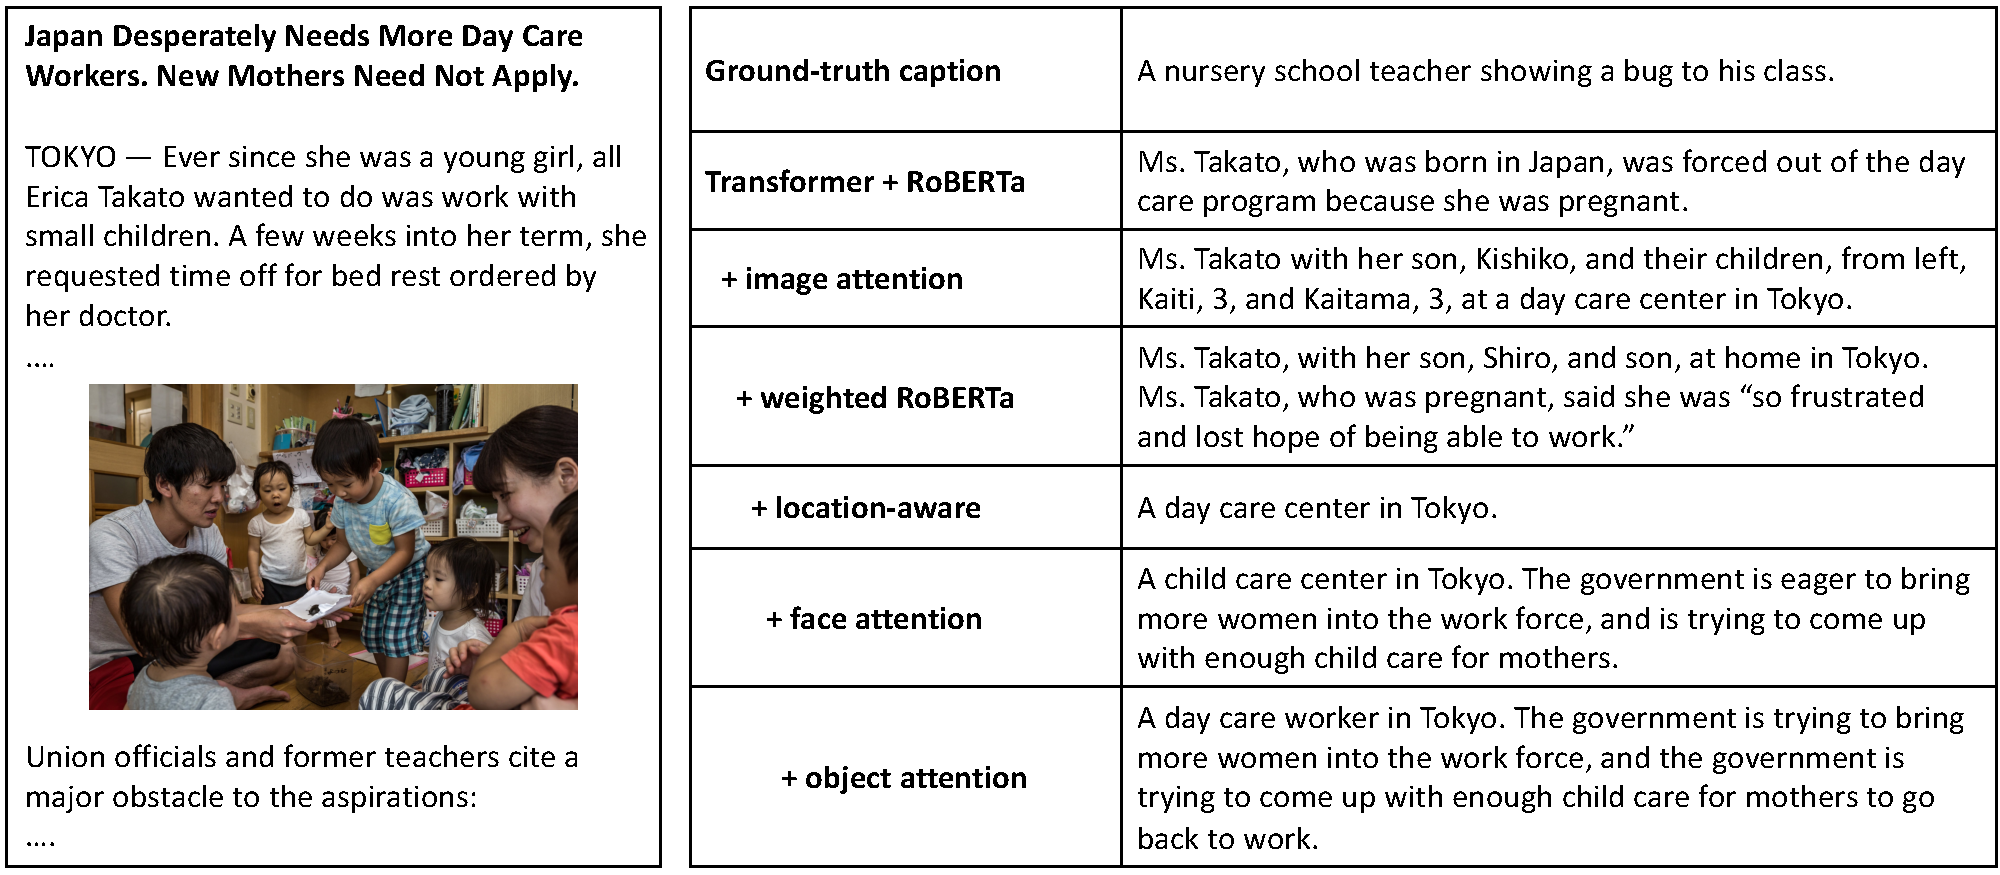
\includegraphics[width=\linewidth]{figures/childcare.pdf}
	\end{center}
	\capmoveup
	\caption{An example article (left) and the corresponding news captions
		(right) from the NYTimes800k test set. The model with no access to the
		image makes a sensible but incorrect guess that the image is about Ms.
		Takato. Since the image appears in the middle of the article, only the
		location-aware models correctly state that the focus of the image is on
		a day care center.}
	\label{fig:example}
	\smallfigmoveup
\end{figure*}

% \eat{\textit{LSTM + GloVe} outperforms this previously state-of-the-art model in
% many metrics (BLEU-4, ROUGE, CIDEr) suggest that using BPE in the decoder
% offers a strong alternative to template-based methods.}

Our most basic LSTM model (row 3) differs from
Biten~\etal~\cite{Biten2019GoodNews} in that we use BPE in the caption decoder
instead of template generation and filling. The slight improvement in CIDEr
(from 13.1 to 13.9) shows that BPE offers a competitive end-to-end alternative
to the template filling method. This justifies the use of BPE in the remaining
experiments.

Models that encode articles using GloVe embeddings (rows 3--4 and 11--12) are
unable to generate rare proper nouns, giving a precision and recall of 0. This
is because the encoder skips words that are not part of the fixed GloVe
vocabulary. This motivates the switch from GloVe to RoBERTa, which has an
unbounded vocabulary. This switch shows a clear advantage in rare proper noun
generation. On NYTimes800k, even the worst performing model that uses RoBERTa
(row 13) achieves a precision of 7.47\%, a recall of 9.50\%, and a CIDEr gap of
12.8 points over the model without RoBERTa (row 11).

Another important modeling choice is the functional form of the caption
decoder. We find that the Transformer architecture provides a substantial
improvement over the LSTM with respect to all evaluation metrics. For example,
when we swap the LSTM with a Transformer (from row 13 to 15), the CIDEr score
on NYTimes800k jumps from 24.9 to 40.3.

\eat{Which is the largest improvement brought by any single modelling choice.}
%% it is not ! BPE encoder has larger gains
%Switching from an LSTM to a transformer architecture improves the
%CIDEr score on NYTimes800k by 8 points, from 12 to 20. If we then use the
%contextualize RoBERTa embeddings instead of GloVe, CIDEr more than doubles
%to 44.

Adding attention over faces improves both the recall and precision of people's
names. It has no significant effect on other entity types (see the
supplementary material for a detailed breakdown). Importantly, people's names
are the most common entity type in news captions and so we also see an
improvement in CIDEr. Attention over objects also improves performance on most
metrics, especially on NYTimes800k. More broadly, this result suggests that
introducing specialized vision models tuned to the common types of objects such
as organizations (via logos or landmarks) is a promising future direction to
improve the performance on news image captioning.

% The word \textit{copying} mechanism leads to a substantial performance
% improvement across all metrics, for example on the NYTimes800k dataset CIDEr
% improves from 54.7 to 65.3. We also see large improvements in the precision and
% recall of rare proper nouns (6.6\% jump in precision and 11.7\% in recall on
% NYTimes800k), as \textit{copying} is designed to handle names that are
% difficult to generate. \eat{for example on the NYTimes800k dataset the
% precision increases from 33.6 to 39.9 with the recall also improving from 26.6
% to 38.3.} This suggests that the \textit{copying} mechanism complements the use
% of BPE, with both techniques contributing to the ability to generating rare
% terms.

The location-aware models (rows 17--19) focus the article context using the
image location in the article, information which is only available in our
NYTimes800k dataset. This simple focusing of context offers a big improvement
to CIDEr, from 45.1 (row 16) to 52.8 (row 17). This suggests a strong
correspondence between an image and the closest text that can be easily
exploited to generate better captions.

%We can make the following observations:

%\begin{itemize}
\eat{\item Our LSTM model with GloVe embeddings outperforms the previous
	state-of-the-art~\cite{Biten2019GoodNews}, indicating that BPE encoding
	offers a viable alternative to template-based methods.}

\eat{ \item Models which encode articles using GloVe embeddings are unable
	to
	generate rare proper nouns (precision and recall of 0).
	This is because the encoder skips words that are not part of the fixed
	GloVe
	vocabulary. Models that use the BPE based article encoder RoBERTa, and thus
	have an unbounded vocabulary show
	a clear advantage in rare proper noun generation, with precision as high as
	38.3\% at a recall of 39.9\%.}



%\end{itemize}

The supplementary material additionally reports three caption quality metrics:
caption length, type-token ratio (TTR)~\cite{Templin1957CertainLS}, and Flesch
reading ease (FRE)~\cite{Flesch1948,Kincaid1975DerivationON}. TTR is the ratio
of the number of unique words to the total number of words in a caption. The
FRE takes into account the number of words and syllables and produces a score
between 0 and 100, where higher means being easier to read. As measured by
FRE, captions generated by our model exhibit a level of language complexity
that is closer to the ground truths. Additionally, captions generated by our
model are 15 words long on average, which is closer to the ground-truths (18
words) than those generated by the previous state of the art (10
words)~\cite{Biten2019GoodNews}.
